%-----------------------------------------------------------------------------
%
%               Template for sigplanconf LaTeX Class
%
% Name:         sigplanconf-template.tex
%
% Purpose:      A template for sigplanconf.cls, which is a LaTeX 2e class
%               file for SIGPLAN conference proceedings.
%
% Guide:        Refer to "Author's Guide to the ACM SIGPLAN Class,"
%               sigplanconf-guide.pdf
%
% Author:       Paul C. Anagnostopoulos
%               Windfall Software
%               978 371-2316
%               paul@windfall.com
%
% Created:      15 February 2005
%
%-----------------------------------------------------------------------------


\documentclass[10pt,nocopyrightspace]{sigplanconf}

% The following \documentclass options may be useful:
%
% 10pt          To set in 10-point type instead of 9-point.
% 11pt          To set in 11-point type instead of 9-point.
% authoryear    To obtain author/year citation style instead of numeric.

\usepackage[normalem]{ulem}
\newcommand{\Comment}[1]{\textcolor{red}{\bf #1}}
%\renewcommand{\iff}{\ensuremath{\mathrm{iff}}}
\usepackage{tabularx}
\usepackage{fancyhdr}
\usepackage{float}
\usepackage{graphicx}
\usepackage[labelfont=bf]{caption}
\usepackage{subcaption}
\usepackage{natbib}
\usepackage{balance}

\begin{document}

%\titlebanner{}        % These are ignored unless
\preprintfooter{}   % 'preprint' option specified.

\title{Automatic Pipeline Synthesis in Chisel}
\subtitle{}

\authorinfo{Huy Vo, Wenyu Tang}
           {University of California, Berkeley}
           {\{huytbvo, wenyu\}@eecs.berkeley.edu}

\maketitle

\section{Introduction}
\cite{Bachrach-2012}

\section{Related Works}
\label{sec:related-work}

Our paper shares the same high level goal as
Halide~\cite{halide:siggraph}: decoupling the algorithm from the
scheduling to simplify the algorithm specification. Halide allows
programmers to write high performance image processing pipelines
without sacrificing readability in a domain-specific language that can
be compiled to different backends. Our pipeline synthesis tool allows
the user to describe a hardware datapath (the algorithm) and the pipeline
specification (the scheduling) for that datapath separately. The
Spiral~\cite{hoe:spiral} hardware generation framework and system
also follows a similar theme. Spiral allows users to generate hardware
for linear transforms from input problem specifications and directives
that describe the datapath. Nurvitadhi et al~\cite{hoe:syn} present
separate tools T-spec for transactional datapath specification and
T-piper for automatic pipeline synthesis. T-spec is used to describe
transactional datapaths as state elements and acyclic next-state logic
blocks that updates those state elements. Users manually annotate all
the state elements and next-stage logic blocks with the pipeline
stage number. T-piper analyzes the T-spec design to identify RAW
hazards and generate hazard resolution logic. Our tool is
different in that the datapath and pipeline specification are both
within the same language. The datapath specification does not have any
notion of stage number and the pipeline specification is maintained
separately from the datapath. Our synthesis tool then takes as input
the datapath and pipeline specification to infer pipeline register
placement and generate the appropriate hazard resolution logic.


\section{Specification}
We utilize Chisel(Constructing Hardware In a Scala Embedded
Language)~\cite{Bachrach:2012} as the basis of our datapath and
pipelining specification. Chisel is an experimental hardware
description language implemented through a set of class definitions
within the high level programming language Scala. Chisel allows for
the designer to fully leverage the high level object oriented
programming features of the Scala language to succinctly describe
hardware. A design described in Chisel can be mapped to a C++
simulator or to Verilog emitted for either FPGA simulation or ASIC
synthesis.

\subsection{Datapath Specification}
The datapath can be specified by a set of architectural state elements
and their next state update logic. We also add a special {\tt Variable
Latency Interface} to allow users to integrate into the datapath
functional units that do not have valid output available every cycle,
such as caches and multi-cycle dividers. In the context of our
specification, Chisel's existing syntax is used to wire up
combinational logic and modules implementing the {\tt Variable Latency
Interface}, which functions as next state logic, to Reg and Transaction
Mem constructs, which function as a single architectural state element
and an addressable array of architectural state respectively.

{\bf Regs}. {\tt Regs} are existing Chisel constructs that represent a
single multi-bit wide flip-flop with synchronous reset and clock
enable ports. They can be treated as single piece of architectural
state that is conditionally updated by every transaction contingent on
the clock enable input.

\begin{figure}[htb]
\centering
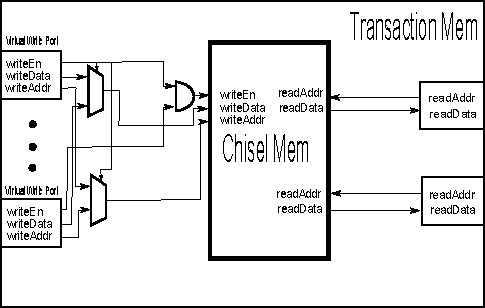
\includegraphics{figures/TMEM.pdf}
\caption{{\bf Transaction Mem} Shows an example of a Transaction Mem with many virtual write ports, one physical write port, and two read ports}
\label{fig:tmem}
\end{figure}

{\bf Transaction Mems}. Transaction Mems are Chisel Components that
wrap existing Chisel Mem constructs in an IO interface that helps the
automatic synthesis tools detect bypassing opportunities. On
instantiation the {\tt Transaction Mem} allows the user to specify the
number of lines in the memory, number of read ports on the IO, number
of virtual write ports on the IO, and the number of physical write
ports on the underlining Chisel Mem construct. Each read port consists
of a read address input and a read data output. There is a one to one
mapping between {\tt Transaction Mem} read ports and underlining read ports
in the Chisel Mem construct. Each virtual write port consists of a
write address input, write enable input, and write data input. The
{\tt Transaction Mem} wrapper automatically maps the virtual write ports on
the IO to the physical write ports of the underlining Chisel Mem
construct. If the number of virtual write ports exceeds the number of
physical write ports, the {\tt Transaction Mem} module automatically
coalesces multiple virtual write ports onto a single physical write
port by muxing together the write data and write addresses of the
virtual write ports and ORing together the write enables of the
virtual write ports. The user should wire each distinct source of
write data along with the associated write enable and write address
into separate virtual write ports rather than manually coalescing the
write data together with a mux and wiring the output of the mux into
a single virtual write port in order to allow the automatic synthesis
tools to generate fine grained bypass logic. This will be elaborated
upon in 4.3.
\begin{figure}[htb]
\centering
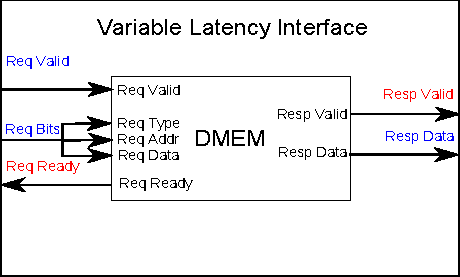
\includegraphics{figures/VLI.pdf}
\caption{{\bf Variable Latency Interface} Blue wires are user facing IO and read wires are tool facing IO.}
\label{fig:vli}
\end{figure}

{\bf Variable Latency Interface}. Variable latency Interfaces are a
Chisel Components that specify a set of user facing IO to allow users
to integrate an existing variable/multi-cycle latency Chisel module
into the datapath specification and a set of tool facing IO to allow
the automatic synthesis tools to generate appropriate pipeline logic
to deal with variable/multi-cycle latency modules. The Variable
Latency Interface exposes on its user facing IO a request ready input,
request data input, and response data output. The user connects the
user facing IO to the rest of the datapath using standard Chisel
syntax. The tool facing IO includes a request ready output and a
response valid output. The tools use the request ready output to
generate logic that puts back pressure on the pipeline stages before
the variable latency module and use the response valid output to
generate logic to insert bubbles into the pipeline stages after the
variable latency module. Figure~\ref{fig:vli}. gives and example of how to
integrate a Data Cache into the datapath specification through
wrapping it in a Variable Latency Interface.

Everything used in the datapath specification is either a built in
Chisel construct(Regs and combinational logic) or a ordinary Chisel
Component({\tt TransactionMems} and {\tt Variable Latency Interfaces}). This
allows the user to create a datapath specification in the exact same
way they would write an ordinary Chisel module, with the exception
that they have to use {\tt TransactionalMems} in place of Mem constructs and
have to wrap up functional units that do not have valid output data
every cycle in {\tt Variable Latency Interfaces}. The datapath specification
by itself, without any pipelining specification, functions as a single
cycle implementation of the datapath.

\subsection {Pipelining Specification}
Once the single cycle datapath has been specified, the user can add
separate annotations to specify how the datapath should be
pipelined. The main parameters in pipelining specification is the
placement of the pipeline registers, the depth of the pipeline, and
how pipeline hazards are resolved.

{\bf Pipeline register placement}. The placement of the pipeline
registers is specified by annotating combinational logic nodes and
read/write ports of the architectural state elements with pipeline
stage numbers. The user can annotate just the big pieces of combinational
logic and architectural state they care about, such as ALUs, register
files, or caches, and the automatic synthesis tool will infer the
placement of all the other parts of the datapath. Of course, the user
gains more control over the placement of the pipeline registers by
adding more pipeline stage annotations. The user can have complete
control over the placement of the pipeline registers if they annotate
every combinational logic node and read/write port in the datapath. The details of the pipeline
register placement are elaborated in section 4.1.

{\bf Pipeline depth}. Pipeline depth is inferred from the maximum
pipeline stage number the user annotates a combinational logic node or
read/write port with.



\section{Automatic Pipeline Synthesis}
\begin{figure*}[htb]
\centering
  \begin{subfigure}[t]{0.8\textwidth}
  \centering
  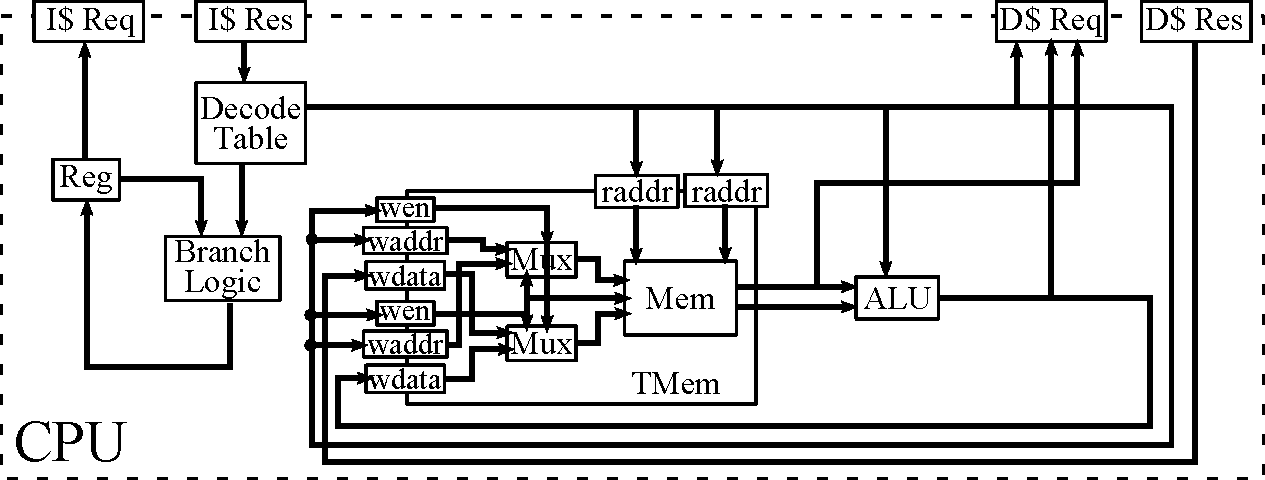
\includegraphics[width=\textwidth]{figures/pipeline.pdf}
  \caption{Datapath Graph.}
  \label{fig:datapathgrah}
  \end{subfigure}
  \begin{subfigure}[t]{0.8\textwidth}
  \vspace{20pt}
  \centering
  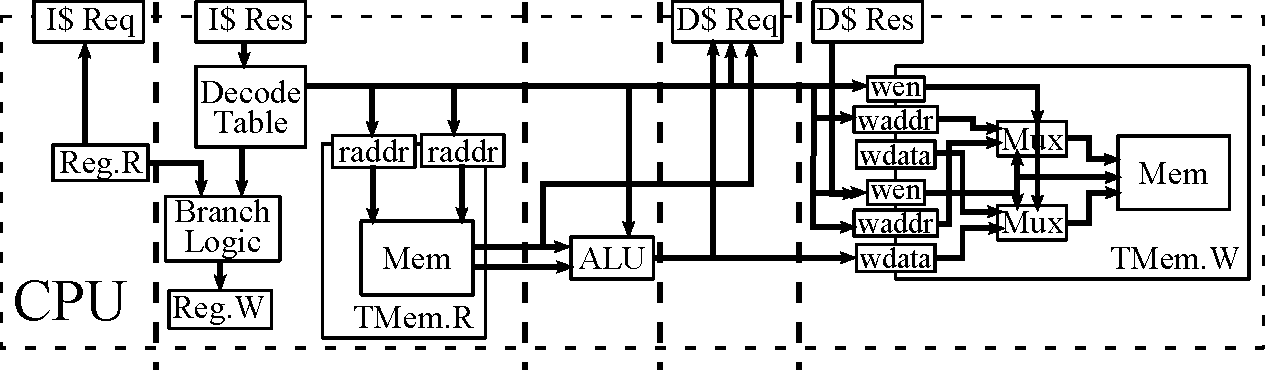
\includegraphics[width=\textwidth]{figures/pipelinedag.pdf}
  \caption{Datapath turned into a DAG.}
  \label{fig:datapathdag}
  \end{subfigure}
\caption{CPU Datapath}
\label{fig:datapath}
\end{figure*}

\subsection{Pipeline Register Placement and Stage Coloring}
{\bf Runtime}. The user annotates a set of combinational logic nodes and architectural state read/write ports with pipeline stage numbers. The user can annotate only the big pieces of combinational logic and architectual state they care about, such as ALUs, register files, or caches, and the automatic synthesis tool will infer the placement of all the other parts of the datapath. Of course, the user gains more control over the placement of the pipeline registers by adding more pipeline stage annotations. The user can have complete control over the placement of the pipeline registers if they annotate every combinational logic node and read/write port in the datapath.

{\bf Elaboration time}. The elaboration time transformation function first breaks the original cyclic Chisel Node graph into an acyclic graph by separating architectual states into read ports and write ports. Then the known pipeline stage numbers from the user annotated Chisel Nodes are propagated to their producers and consumers in a pseudo breadth-first-search(BFS) manner. When two propagation frontiers meet at the same node, propagation down that path stops and pipeline registers are inserted at that node. We also record the stage numbers of all Chisel Nodes after the stage propagation and pipeline register insertion for use in detecting pipeline hazards in the next stage of the automatic pipeline synthesis.

{\bf Pipeline Stage Propagation Details}. Nodes and their stage numbers are kept track of in a map of Nodes to List of Stage Numbers that we will refer to as the stage number map. Initially, only the user annotated nodes have non-empty values in the stage number map. In the pseudo BFS traversal, the propagation frontier(ie the nodes that have yet to propagate out their stage numbers) is kept track of with a queue. The propagation frontier queue is initialized with the user annotated nodes. As with a normal BFS traversal, the head of the propagation frontier queue is dequeued, some visit operation is performed on the dequeued node, and its children, which includes both producers and consumers, are enqueued onto the propagation frontier queue. Unlike a normal BFS traversal, the dequeued node maybe re-enqueued by the visit operation. In this case, the visit operation tries to propagate out the stage number of the dequeued node to its children by appending the dequeued node's stage number to its children's stage number list in the stage number map if the node is not the meeting point of two propagation frontiers, but re-enqueues the node for a retry later if it is not currently possible to propagate out the node's stage number. The node can propagate out its stage number if the following conditions are true: (1) the node has exactly one stage number in its stage number list in the stage number map and (2) all of the nodes children are ready to receive a stage number. 

Condition (1) makes sure that the propagation front has reached the node, which means that the node has atleast one stage number in its stage number list, and that two propagation frontiers have not meet at that node, which would mean that the node has less than 2 stage numbers in its stage number list. 

Condition (2) makes sure that the node propagates out its stage number to all of its children in an atomic manner. This is necessary because the propagation would produce incorrect results if the node managed to propagate out its stage number to only some of its children before two propagation frontiers meet at that node and stop the node from propagating its stage to the rest of its children. The node can only propagate its stage number to all of its children atomically if it waits until all of its children are ready and propagates to all of them at the same time, before the next node dequeued from the propagation frontier queue. The next paragraph discusses why some children may not be immediately ready to receive a stage number propagation.

We need to check that nodes are ready to receive a stage number because we need to enforce that a node has a stage number >= the stage numbers of all of its producer nodes and <= the stage numbers for all of its consumer nodes. For nodes with multiple producers, such as combinational logic nodes, the stage number propagated to the node from the producer side should be the maximum of the stage numbers of all of its producers. Also for nodes with multiple consumers the stage number propagated to the node from the consumer side should be minimum of the stage number of all its consumers. Thus, a node is ready to receive a stage number propagation from its producer side if a propagation frontier has reached all of its producer nodes and a node is ready to receive a stage number propagation from its producer side if a propagation frontier has reached all of its consumer nodes.

Once the stage number propagation is complete, we traverse the Chisel Node graph again and insert the appropriate number of pipeline registers between any adjacent nodes with different stage numbers and on any nodes with more than one stage number in its stage numbers list in the stage numbers map. Refer to [figure xx] for pseudo code on the stage number propagation algorithm.
\subsection{Hazard Discussion}
\begin{figure*}[htb]
\centering
  \begin{subfigure}[t]{0.8\textwidth}
  \centering
  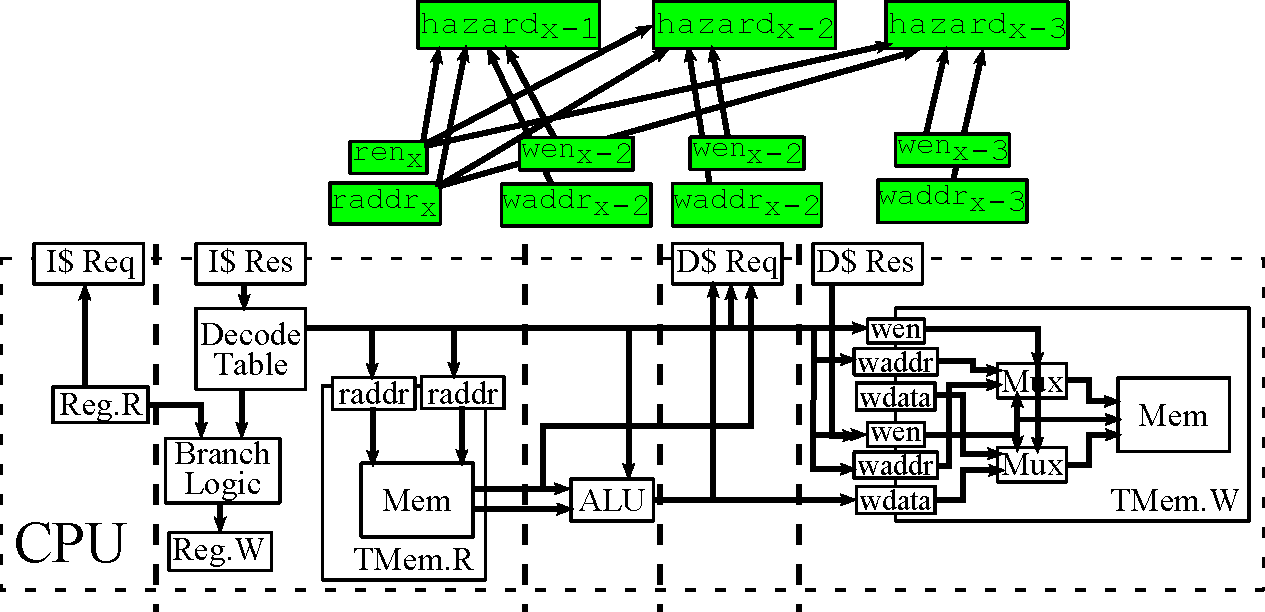
\includegraphics[width=\textwidth]{figures/pipelinehazard.pdf}
  \caption{Hazard Detection.}
  \label{fig:haz}
  \end{subfigure}
  \begin{subfigure}[t]{0.8\textwidth}
  \vspace{20pt}
  \centering
  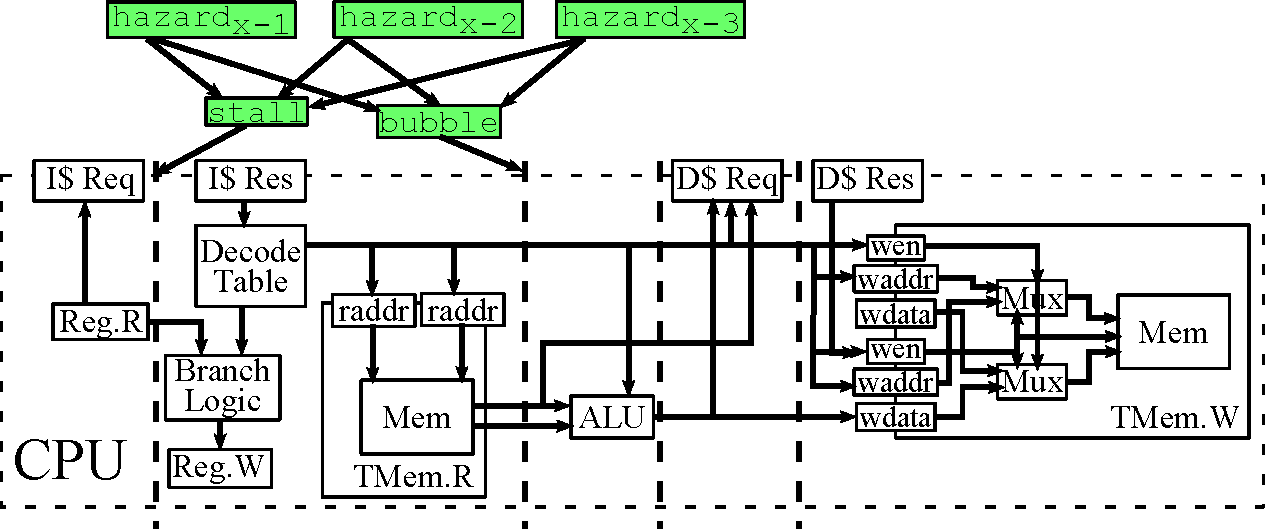
\includegraphics[width=\textwidth]{figures/pipelineinterlock.pdf}
  \caption{Interlocks.}
  \label{fig:int}
  \end{subfigure}
\caption{Resolving hazards through interlocks}
\label{fig:hazint}
\end{figure*}

{\bf Hazard Types}.

{\bf Detection}. Inserting pipeline registers into the datapath
graph introduces pipelining hazards that are not present in the
unpipelined datapath. Here we discuss how to handle data hazards which
result from a transaction reading a state element (a {\tt Reg} node or a
{\tt TransactionalMem}) before an earlier transaction writes to that state
element. 

We first search through the datapath graph to find all state
elements. For every state element, we determine whether or not a
hazard exists on it. If there is a hazard on a state element, we add
the hazard condition into a list. For {\tt Reg} or {\tt TransactionalMem}, a
hazard condition exists if the state element belongs in a stage that precedes the
stage of its write enable or write data signal. The actual Boolean
hazard condition is {\tt wen \&\& ren} for a {\tt Reg} node and
{\tt wen \&\& ren \&\& waddr == raddr} for a {\tt TransactionalMem}.

Figure~\ref{fig:haz} shows the hazard conditions that our tool
identifies on the {\tt TransactionalMem}. when analyzing the generated pipeline in
Figure~\ref{fig:datapathdag}. We first search the pipeline for all
state elements. In this example, the {\tt Reg} node and the 
{\tt TransactionalMem} are the only state elements. We then examine
the read and write ports of these state elements to determine whether
or not there are any hazards. The {\tt Reg} has its write port in the
second stage but its read port is in the first stage. So we generate a
hazard signal in the first stage. The {\tt Transactionalmem} has its
write port in the fifth stage but its read port is in the second
stage. We trace backwards from the {\tt wen} in the fifth stage to the
second stage to find all the other {\tt wen} signals. For each 
({\tt wen}$_i$, {\tt waddr}$_i$) pair, we generate a hazard condition
{\tt wen$_i$ === ren$_i$ \&\& waddr$_i$ === raddr}.

\subsection{Hazard Resolution Options}
\begin{figure*}[htb]
\centering
  \begin{subfigure}[t]{0.8\textwidth}
  \centering
  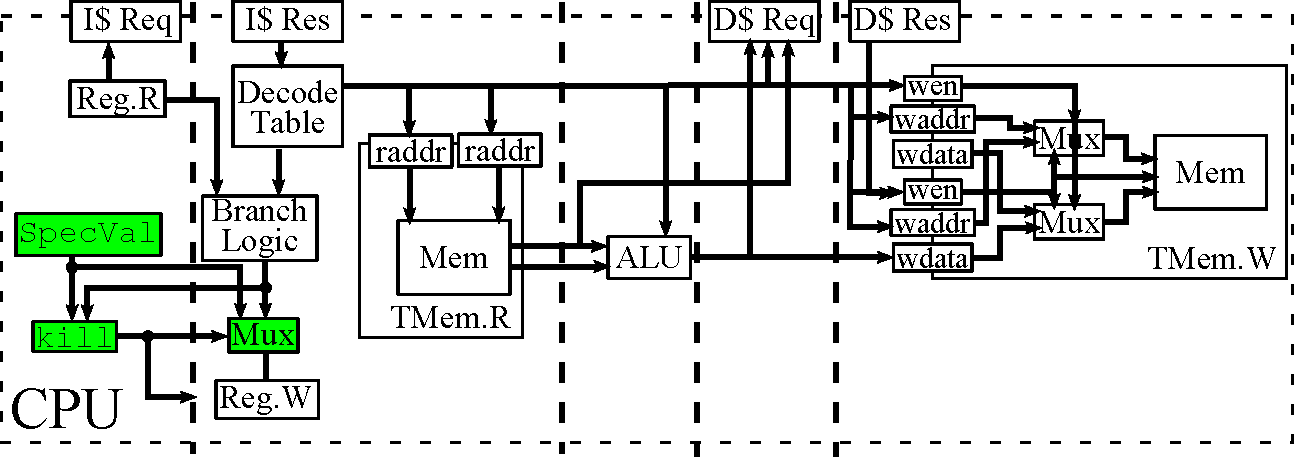
\includegraphics[width=\textwidth]{figures/pipelinespec.pdf}
  \caption{Speculation.}
  \label{fig:spec}
  \end{subfigure}
  \begin{subfigure}[t]{0.8\textwidth}
  \vspace{20pt}
  \centering
  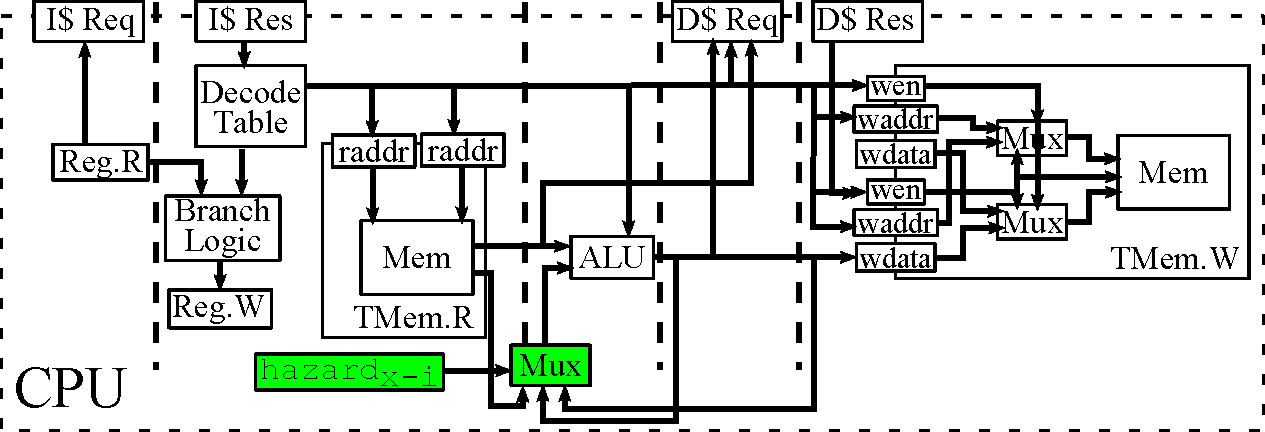
\includegraphics[width=\textwidth]{figures/pipelinebypass.pdf}
  \caption{Bypassing.}
  \label{fig:bypass}
  \end{subfigure}
\caption{Resolving hazards through speculation and bypassing}
\label{fig:specbyp}
\end{figure*}

{\bf Interlocks}. The easiest way to resolve
hazards is through interlocks. This hazard resolution method requires
no additional input from the user. Every identified hazard is placed
into the stage of the read port that generates the hazard. In
Figure~\ref{fig:haz}, the hazards would be placed into the second
stage because the corresponding read port is in the second stage. We
then go through every stage and perform an {\tt OR} reduction on all
the hazards in that stage as well as all the hazard conditions in the
following stages to produce the stall condition for that stage. The
second part of interlocking a pipeline is to push bubbles. We go
through every stage and generate a {\tt pushBubble} signal if there is
a hazard condition in that stage and no following stages have a
hazard.

Figure~\ref{fig:int} shows the interlock logic that our tool
generates to handle the hazards from Figure~\ref{fig:haz}. Since
the {\tt TransactionalMem}'s read port is in the second stage, all the
{\tt hazard$_i$}s go into the second stage. When examining the second
stage, the tool would {\tt OR} reduce all the {\tt hazard}$_i$s to
generate a stall condition to stall the first stage. The same hazard
condition is then used to generate the {\tt pushBubble} signal. There
are no other sources of hazards further down the pipeline so the
hazard condition in the second stage is sufficient for pushing a
bubble into the second stage.

{\bf Speculation}.

{\bf Bypassing}.

\section{Results}
\begin{figure*}[htb]
\centering
  \begin{subfigure}[t]{0.47\textwidth}
  \centering
  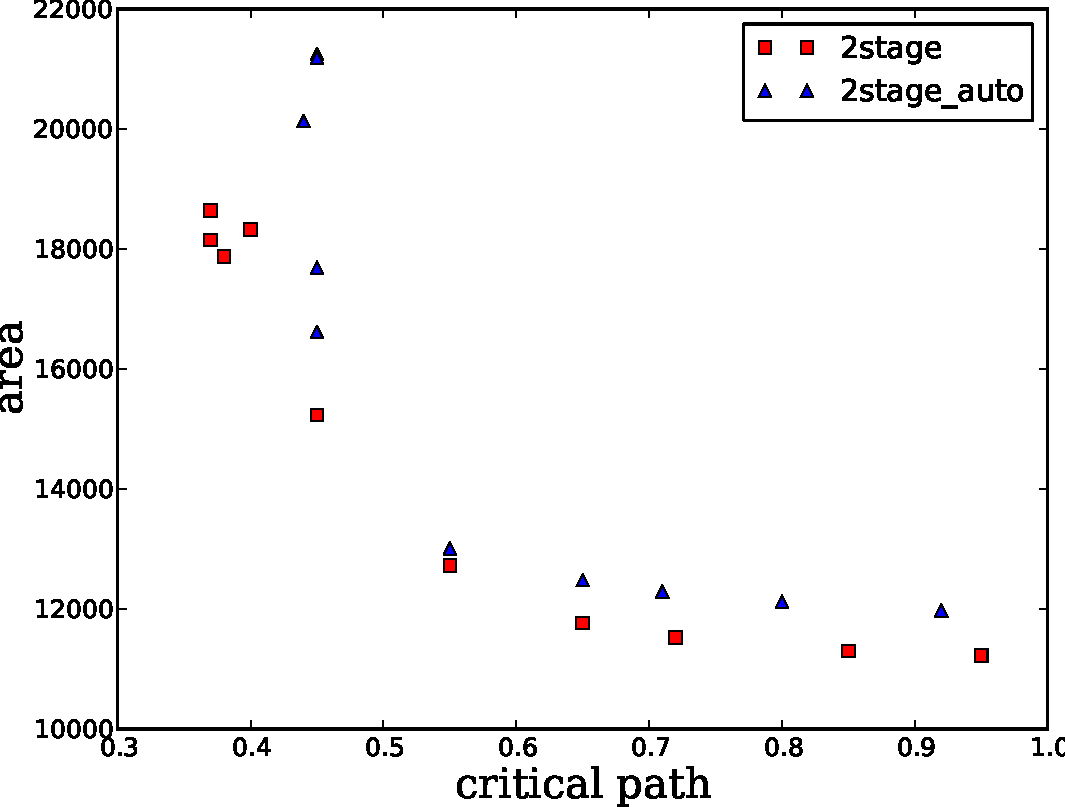
\includegraphics[width=\textwidth]{figures/2stage.pdf}
  \caption{2-stage}
  \label{fig:2stage}
  \vspace{20pt}
  \end{subfigure}
  \hfill
  \begin{subfigure}[t]{0.47\textwidth}
  \centering
  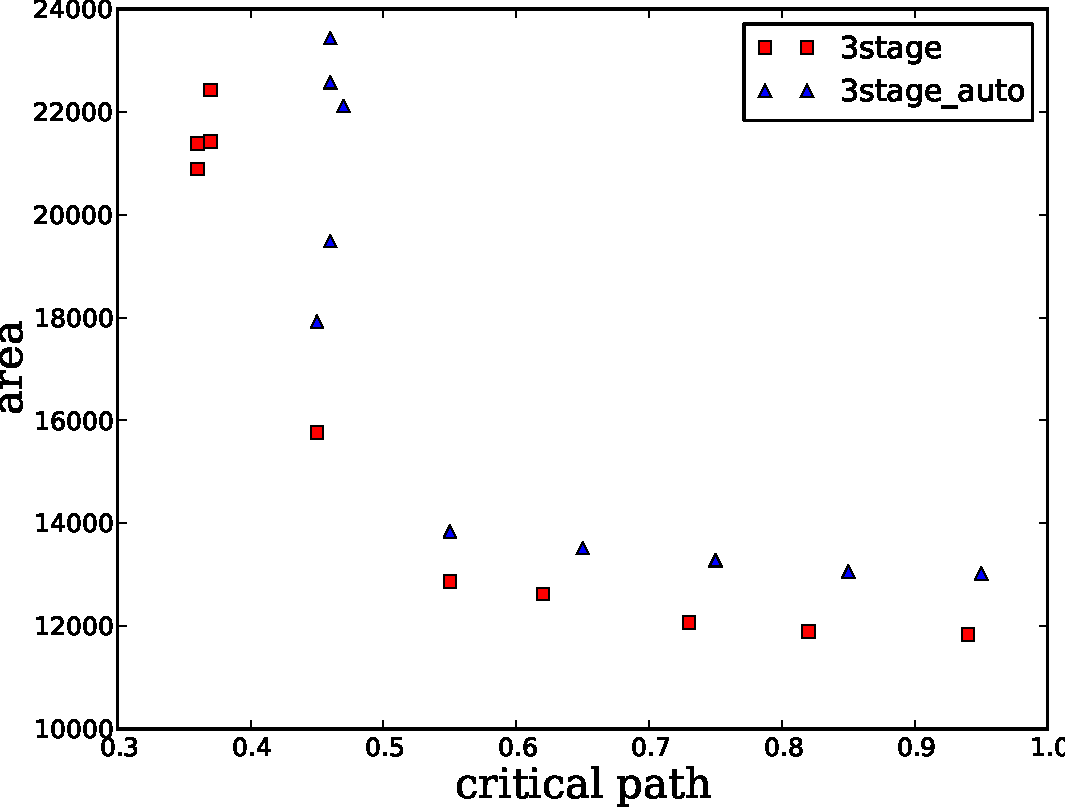
\includegraphics[width=\textwidth]{figures/3stage.pdf}
  \caption{3-stage}
  \label{fig:3stage}
  \vspace{20pt}
  \end{subfigure}
  \hfill
  \begin{subfigure}[t]{0.47\textwidth}
  \centering
  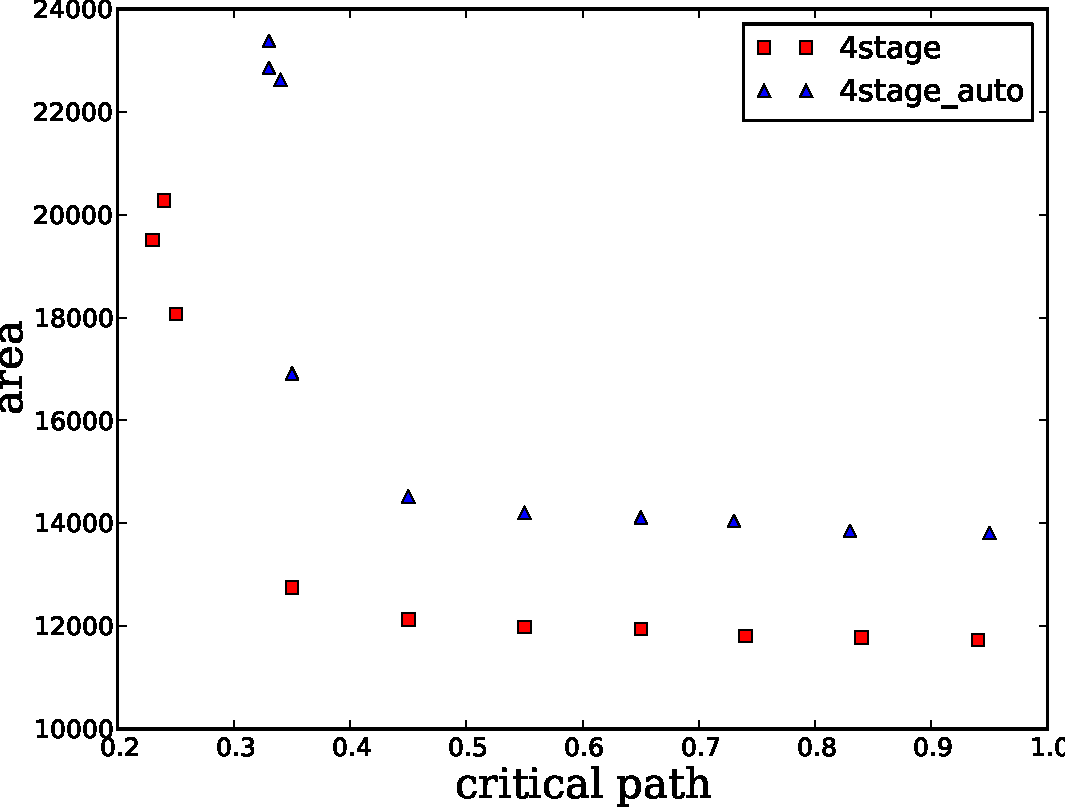
\includegraphics[width=\textwidth]{figures/4stage.pdf}
  \caption{4-stage}
  \label{fig:4stage}
  \end{subfigure}
  \hfill
  \begin{subfigure}[t]{0.47\textwidth}
  \centering
  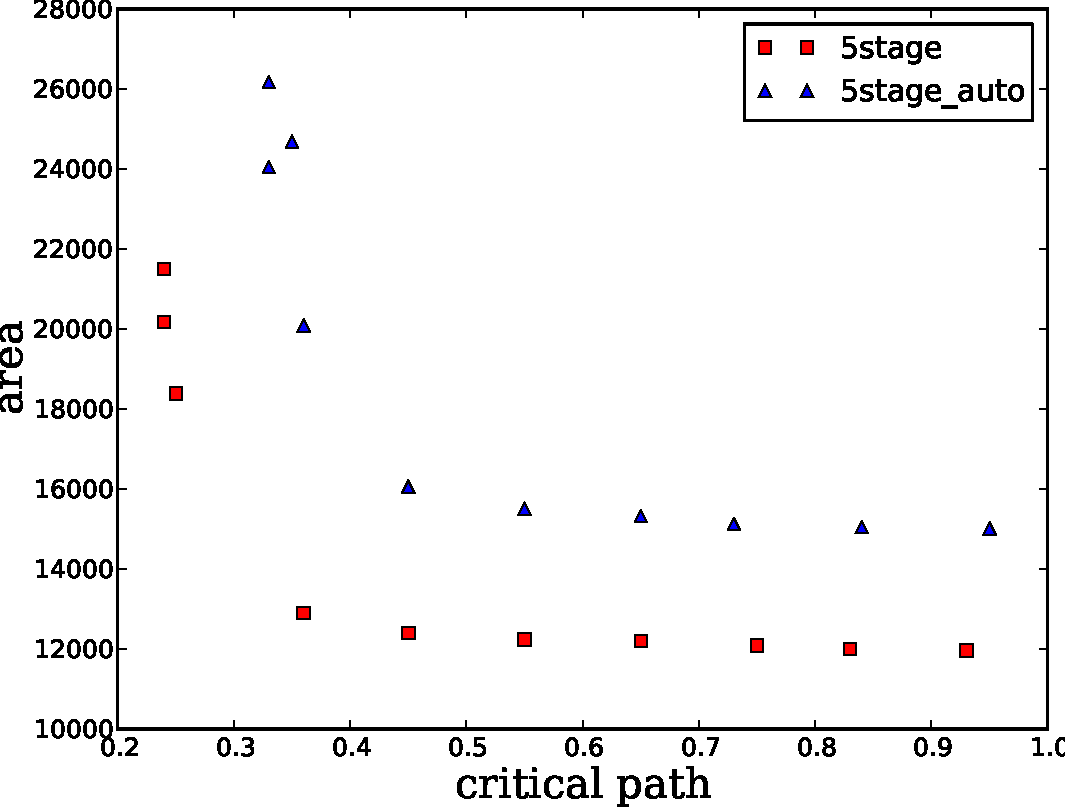
\includegraphics[width=\textwidth]{figures/5stage.pdf}
  \caption{5-stage}
  \label{fig:5stage}
  \end{subfigure}
\caption{{\bf Area vs Critical Path Comparison}. Area is measured in
  square micron. Critical path is measured in nanosecond.}
\label{fig:area-time}
\end{figure*}
\begin{figure*}[htb]
\centering
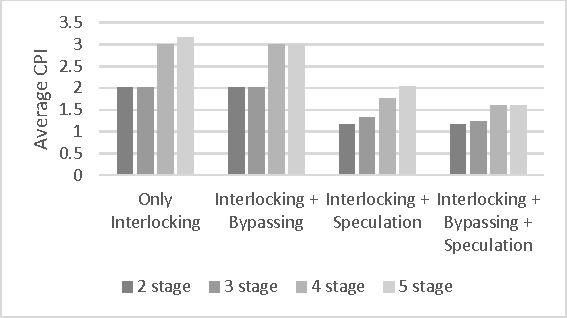
\includegraphics[trim = 25mm 190mm 100mm 0mm, clip]{figures/cpi.pdf}
\caption{{\bf CPI} averaged over the median, mixed-manufacturing, multiply, qsort, towers, and vvadd benchmarks.}
\label{fig:CPI}
\end{figure*}
To evaluate our pipeline synthesis tool, we write a 2-stage, 3-stage,
4-stage, and 5-stage pipeline specification for a single cycle CPU
datapath. We present CPI results to show that our synthesis tool is
effective in improving performance. We also push our auto-generated
pipeline through Design Compiler synthesis tool using TSMC's 45nm CMOS
library and compare the post-synthesis results to hand-coded 2-stage,
3-stage, 4-stage, and 5-stage pipelines.
\subsection{CPI}
As shown by Figure[xx], our synthesis tool does indeed improve performance by utilizing speculation and bypassing as expected. The 2-stage and 3-stage CPUs have their branches resolved in the 2nd pipeline stage and the 4-stage and 5-stage CPUS have their branches resolved in the 3rd pipeline stage. Speculation is is performed on the PC register and bypassing is performed on both read ports of the register file. There is little performance improvement from turning on bypassing without turning on speculation because most of the RAW hazards on the register file are covered up by interlocks on the PC register.
\subsection{Sodor}
Sodor is a set of simple processors written in Chisel. We use Sodor's
1-stage processor for the datapath specification. In order to work
with our tool, we modify the 1stage to use {\tt TransacationalMem}
instead of {\tt Mem} and wrapped the instruction and data cache with
our variable latency interface. Sodor also provides 2 and 5-stage
in-order processor that we use to compare against our auto-generated 2
and 5-stage processor. We had to write a 3-stage and 4-stage processor
ourselves. The hand-coded 2-stage has speculation on the PC
register. The 3, 4, and 5-stage processors make use of speculation on
the PC register and bypassing to forward results from the ALU and the
data cache.

\subsection{Comparison}
In order to see how our auto-generated pipeline holds up against a
hand-written pipeline, we push the pipelines through
synthesis. Figure~\ref{fig:area-time} compares post-synthesis results
between auto-generated pipelines and their hand-written
counterparts. We push only the CPU portion (datapath and control path,
no caches) of the processor through synthesis to better highlight the
overhead of our pipeline synthesis tool. Figure~\ref{fig:2stage} and
Figure~\ref{fig:3stage} shows that for shorter pipelines our synthesis
tool introduces little overhead. This is due to the fact that there is
very little freedom for placing pipeline registers and there are not
that many hazards to resolve. Our tool performs much worse for larger
pipelines (Figure~\ref{fig:4stage} and Figure~\ref{fig:5stage}) since
there is more freedom for register placement (which could cause our
tool to place more registers than needed) and because there are more
hazards to resolve. In particular, the 4 and 5-stage pipelines have
more bypass locations. Our tool generates an entire set of muxes for
each of these write paths instead of coalescing these write paths and
using only one mux as in the hand-coded versions.

\section{Conclusion}


\bibliographystyle{abbrvnat}
\setlength{\bibsep}{0.0pt}
\renewcommand*{\bibfont}{\footnotesize}
\bibliography{references}

\end{document}
